\documentclass{article}

\usepackage{array}
\usepackage{graphicx}

\begin{document}

\title{Week 12, Session 1 Problems}
\author{GSI: Caleb Eades}
\date{11/6}
\maketitle

\section{Charges and Magnetic Fields}

\subsection{Mass Spectrometer}

An ion of mass m and charge $+q$ is produces at rest in source S and accelerated across a potential difference $V_0$ and enters a magnetic field B as shown below. The ion moves in a semicircular path and strikes a plate at a distance x from the entrance slit. show that the mass of the ion can be found by the following equation:
\begin{equation}
m=\frac{B^2q}{8V_0}x^2
\end{equation}

\begin{figure}[h]
\begin{center}
	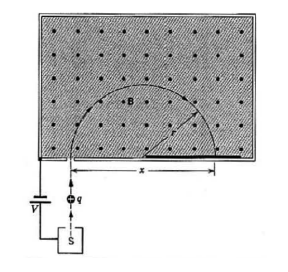
\includegraphics[width=0.5\textwidth]{Spectrometer.png}
\end{center}
\end{figure}

\textit{(Source: modified from Halliday, Chapter 34-4, problem 22)}

\subsection{Forces on Bent Wires}

Find the net magnetic force on the whole wire of current $I$ which consists of two straight segments of length $L$ and a half circular segment of radius $R$ as shown below. The magnetic field is constant and in the $\hat{z}$ direction.

\begin{figure}[h]
	\begin{center}
		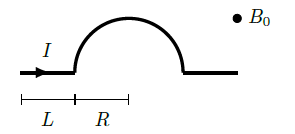
\includegraphics[width=0.5\textwidth]{WireLoop.png}
	\end{center}
\end{figure}

\textit{(Source: Dan Parker and Vetri Velan)}

\subsection{Magnetic Suspension Magic}

A rectangular loop of wire, supporting a mass $m$, hangs vertically with one end in a uniform magnetic field $\vec{B}$, which points into the page in the shaded region of the figure. 
\begin{itemize}
	\item[(a)] For what current $I$ in the loop would the magnetic force upwards exactly balance gravity downwards? 
	\item[(b)] Now suppose we increase the current. Then the magnetic force up exceeds gravity and the weight is lifted. But \textit{magnetic fields do no work}, so how does this happen? Clearly, \textit{something} must be doing work on the mass --- what is it?
\end{itemize}

\begin{figure}[h]
	\begin{center}
		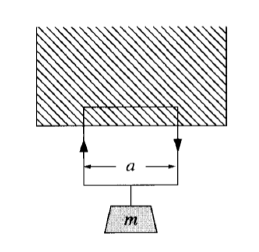
\includegraphics[width=0.3\textwidth]{Suspension.png}
	\end{center}
\end{figure}

\textit{Source: Griffiths EM, Example 5.3}

\subsection{Non-Uniform Fields}

Suppose we have a bent wire that starts at $(x,y,z)=(0,0,L/2)$, goes straight to the origin and then goes straight out to $(x,y,z)=\frac{1}{\sqrt{2}}(L/2,L/2,0)$. If this wire carries current $I$ in that specified direction and there is a magnetic field $\vec{B}=B_0(x\hat{x}+sin(\frac{4\sqrt{2}\pi}{L}y)\hat{y}+z^2\hat{z})$, what is the net force on the wire?

\end{document}
